%%%%%%%%%%%%%%%%%%%%%%%%%%%%%%%%%%%%%%%%%%%%%%%%%%%%%%%%%%%%%%%%%%%%%%%%%%%%%%%%%%%%%%%%%%%%%%%%
%
% CS484 Written Question Template
%
% Acknowledgements:
% The original code is written by Prof. James Tompkin (james_tompkin@brown.edu).
% The second version is revised by Prof. Min H. Kim (minhkim@kaist.ac.kr).
%
% This is a LaTeX document. LaTeX is a markup language for producing 
% documents. Your task is to fill out this document, then to compile 
% it into a PDF document. 
%
% 
% TO COMPILE:
% > pdflatex thisfile.tex
%
% If you do not have LaTeX and need a LaTeX distribution:
% - Personal laptops (all common OS): www.latex-project.org/get/
% - We recommend latex compiler miktex (https://miktex.org/) for windows,
%   macTex (http://www.tug.org/mactex/) for macOS users.
%   And TeXstudio(http://www.texstudio.org/) for latex editor.
%   You should install both compiler and editor for editing latex.
%   The another option is Overleaf (https://www.overleaf.com/) which is 
%   an online latex editor.
%
% If you need help with LaTeX, please come to office hours. 
% Or, there is plenty of help online:
% https://en.wikibooks.org/wiki/LaTeX
%
% Good luck!
% Min and the CS484 staff
%
%%%%%%%%%%%%%%%%%%%%%%%%%%%%%%%%%%%%%%%%%%%%%%%%%%%%%%%%%%%%%%%%%%%%%%%%%%%%%%%%%%%%%%%%%%%%%%%%
%
% How to include two graphics on the same line:
% 
% \includegraphics[\width=0.49\linewidth]{yourgraphic1.png}
% \includegraphics[\width=0.49\linewidth]{yourgraphic2.png}
%
% How to include equations:
%
% \begin{equation}
% y = mx+c
% \end{equation}
% 
%%%%%%%%%%%%%%%%%%%%%%%%%%%%%%%%%%%%%%%%%%%%%%%%%%%%%%%%%%%%%%%%%%%%%%%%%%%%%%%%%%%%%%%%%%%%%%%%

\documentclass[11pt]{article}

\usepackage[english]{babel}
\usepackage[utf8]{inputenc}
\usepackage[colorlinks = true,
            linkcolor = blue,
            urlcolor  = blue]{hyperref}
\usepackage[a4paper,margin=1.5in]{geometry}
\usepackage{stackengine,graphicx}
\usepackage{fancyhdr}
\setlength{\headheight}{15pt}
\usepackage{microtype}
\usepackage{times}
\usepackage{booktabs}
\usepackage{listings}
\usepackage{xcolor}
\lstdefinestyle{codestyle}{
	frame=single,
	basicstyle=\ttfamily\footnotesize,
	keywordstyle=\bfseries\color{magenta},
	commentstyle=\itshape\color{gray},
	stringstyle=\color{orange},
	numberstyle=\sffamily\scriptsize\color{gray},
	showspaces=false,
	showstringspaces=false,
	showtabs=false,
	tabsize=4,
	breakatwhitespace=false,
	breaklines=true,
	keepspaces=true,
	captionpos=b,
	numbers=left,
	numbersep=5pt}
\lstset{style=codestyle}

\frenchspacing
\setlength{\parindent}{0cm} % Default is 15pt.
\setlength{\parskip}{0.3cm plus1mm minus1mm}

\pagestyle{fancy}
\fancyhf{}
\lhead{Homework Writeup}
\rhead{CS484}
\rfoot{\thepage}

\date{}

\title{\vspace{-1cm}Homework 3 Writeup}


\begin{document}
\maketitle
\vspace{-3cm}
\thispagestyle{fancy}

\section*{Instructions}
\begin{itemize}
  \item Describe any interesting decisions you made to write your algorithm.
  \item Show and discuss the results of your algorithm.
  \item Feel free to include code snippets, images, and equations.
  \item \textbf{Please make this document anonymous.}
\end{itemize}

\section*{Bayer Image Interpolation}

First part of this project is to make the code that interpolating the given bayer image into proper RGB image. 

\begin{lstlisting}[language=python]
def bayer_to_rgb_bilinear(bayer_img):
    
    height, width = bayer_img.shape
    rgb_img = np.zeros((height + 2, width + 2, 3), dtype=np.uint8)
    # added zero padding of 1 pixel width around the image for calculation efficiency    
    # Extract bayer image into each channel of rgb image
    # Range starts from 1 due to the padding
    rgb_img[1:-1:2, 1:-1:2, 0] = bayer_img[0::2, 0::2]    
    rgb_img[1:-1:2, 2:-1:2, 1] = bayer_img[0::2, 1::2]
    rgb_img[2:-1:2, 1:-1:2, 1] = bayer_img[1::2, 0::2]
    rgb_img[2:-1:2, 2:-1:2, 2] = bayer_img[1::2, 1::2]

    # For the R channel
    rgb_img[1:height:2, 2:width+1:2, 0] = (rgb_img[1:height:2, 1:width:2,0]//2 + 
    rgb_img[1:height:2, 3:width+2:2,0]//2) 
    rgb_img[2:height+1:2, 1:width:2, 0] = (rgb_img[1:height:2, 1:width:2,0]//2 + 
    rgb_img[3:height+2:2, 1:width:2,0]//2) 

    rgb_img[2:height+1:2, 2:width+1:2, 0] = (
        rgb_img[1:height:2, 1:width:2, 0]//4 + rgb_img[1:height:2, 3:width+2:2, 0]//4 +
        rgb_img[3:height+2:2, 1:width:2, 0]//4 + rgb_img[3:height+2:2, 3:width+2:2, 0]//4
    ) 
    #For the G channel
    rgb_img[1:-1:2, 1:-1:2, 1] = (
        rgb_img[1:-1:2, 0:-2:2, 1]//4 + 
        rgb_img[0:-2:2, 1:-1:2, 1]//4 +
        rgb_img[2::2, 1:-1:2, 1]//4 + 
        rgb_img[1:-1:2, 2::2, 1]//4
    )
    rgb_img[2:height+1:2, 2:width+1:2, 1] = (
        rgb_img[2:height+1:2, 1:width:2, 1]//4 + 
        rgb_img[1:height:2, 2:width+1:2, 1]//4 +
        rgb_img[3:height+2:2, 2:width+1:2, 1]//4 + 
        rgb_img[2:height+1:2, 3:width+2:2, 1]//4
    )

    # For the B channel
    rgb_img[2::2, 1:-2:2, 2] = (rgb_img[2::2, 0:-3:2,2]//2 +
    rgb_img[2::2, 2:-1:2,2]//2) 
    
    rgb_img[1:-2:2, 2::2, 2] = (rgb_img[0:-3:2, 2::2,2]//2 +
    rgb_img[2:-1:2, 2::2,2]//2) 
    
    rgb_img[1:-2:2, 1:-2:2, 2] = (
        rgb_img[0:-3:2, 0:-3:2, 2]//4 + 
        rgb_img[0:-3:2, 2:-1:2, 2]//4 +
        rgb_img[2:-1:2, 0:-3:2, 2]//4 + 
        rgb_img[2:-1:2, 2:-1:2, 2]//4
    )    
    #Remove Padding
    rgb_img = rgb_img[1:-1, 1:-1, :]
    
    return rgb_img
    \end{lstlisting}


\section*{Interesting Implementation Detail}

I'll explain my code step by step. 


\begin{enumerate}
    \item First, I made the empty array for result image with 2 pixels bigger than bayer image. This is because I wanted to add zero padding of 1 pixel around the image, for edge calculation.
    \item Then I brought the each R,G,B pixels from the bayer image and applied to channels in R,G,B order. To apply padding, i left the first and last pixels zero and filled the pixel value starting from 1.
    \item For each channel, used bilinear interpolation to fill the missing pixel values. I used indexing and slicing of Numpy to do this, since it is much faster than naive for loops.
    \item For the pixels in edges, I just used the same ways with other pixels, the only difference is that averaged the zero padding together. This makes the edge value smaller than intended, but it could the code more precise.
    \item Finally, I removed the zero padding by slicing the result image from the first pixel to the second last pixel.
\end{enumerate}

These are two images obatained from bilinear interpolation.

\begin{figure}
    \centering
    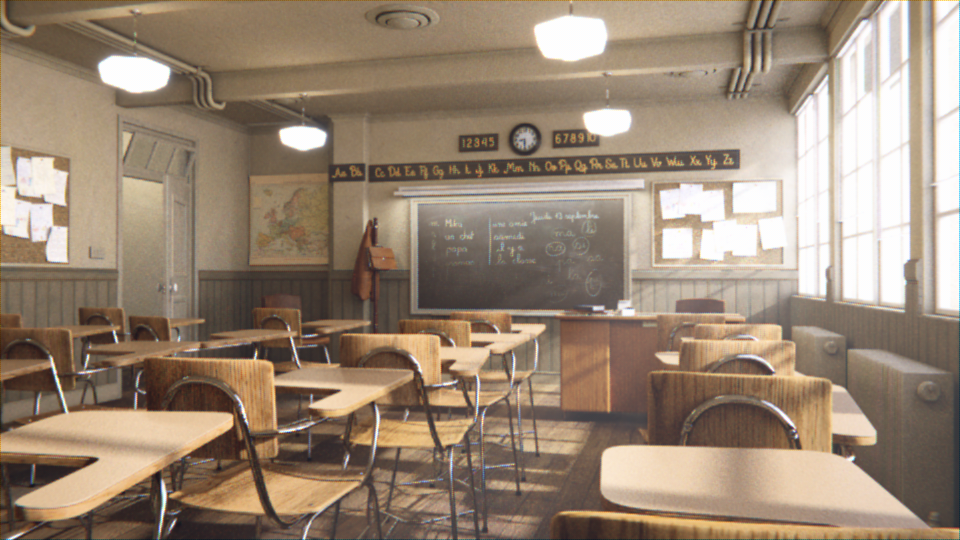
\includegraphics[width=5.5cm]{../result/bilinear_img1.png}
    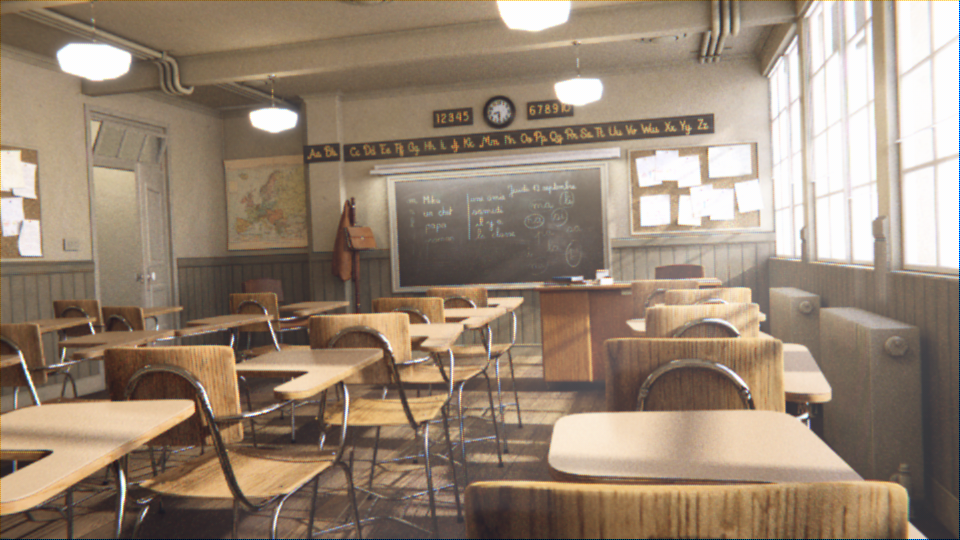
\includegraphics[width=5.5cm]{../result/bilinear_img2.png}
\caption{Images obtained from bilienear interpolation}
\end{figure}

The problem in this implementation is as mentioned, the edge control. I think this could be resolved by using other methods for edges, such as reflection.


\section*{Fundamental Matrix Calculation}
In this section, with given 8 points on both images I obtained the fundamental matrix, using eight-point algorithm.

\begin{lstlisting}[language=python]
def calculate_fundamental_matrix(pts1, pts2):
    assert pts1.shape[1] == 2 and pts2.shape[1] == 2
    assert pts1.shape[0] == pts2.shape[0]
    
    n = pts1.shape[0]
    
    
    pts1_normalized, T1 = normalize_points(pts1.T, 2)
    pts2_normalized, T2 = normalize_points(pts2.T, 2)
    
    # Transpose back to original structure
    pts1_normalized = pts1_normalized.T
    pts2_normalized = pts2_normalized.T
    
    A = np.zeros((n, 9))
    for i in range(n):
        x1, y1 = pts1_normalized[i]
        x2, y2 = pts2_normalized[i]
        A[i] = [x1*x2, x2*y1, x2, y2*x1, y1*y2, y2, x1, y1, 1]
    
    U, S, Vt = np.linalg.svd(A)
    f = Vt[-1]
    F = f.reshape(3, 3)
    
    U, S, Vt = np.linalg.svd(F)
    S[-1] = 0
    F = U @ np.diag(S) @ Vt
    
    # Denormalize
    F = T2.T @ F @ T1
    
    return F
\end{lstlisting}
\begin{enumerate}
    \item \textbf{Normalization}
    First, I normalized the given points using the built-in fuction $normalize\_points()$. Since the function needs input coordinates with x,y in column, I transposed the given points vector and applied the function.
    Then I transposed the result of function to obtain original structure.
    
    \item \textbf{Constructing Matrix A}
    Matrix $A$ is constructed using the normalized points. I just simply put each values in the matrix, and the values come from what we learned in class and supplementary slides.
    
    \item \textbf{Singular Value Decomposition and Reshaping f}
    Performed singular value decomposition for matrix $A$, to obtain $f$.Since $f$ corresponds to the eigenvector of $A^TA$ with the smallest eigenvalue, I extracted the last row of $Vt$. Then, reshaped it into 3x3 matrix. Matrix $F$ is 3x3 fundmental matrix obtained from SVD.
    
    \item \textbf{Enforce F to have Rank 2, and Recalculate F}
    Performed singular value decomposition again for matrix $F$. To enforce rank 2 condition, I set the last row of S(minimum sigular value) zero and recalculated $F$ with new S.
    
    \item \textbf{Denormalization}
    Finally, I denormalized fundamental matrix $F$ with scaling matrix $T1$ and $T2$ to bring it back to the scale of the original points.
\end{enumerate}

\section*{Stereo Rectification}

\section*{Calculating Disparity Map}
The final, and the most complex part of this project is cacluating the disparity map.
\begin{lstlisting}[language=python]
def calculate_disparity_map(img1, img2):
    
    # First convert color image to grayscale
    img1_gray = cv2.cvtColor(img1, cv2.COLOR_RGB2GRAY)
    img2_gray = cv2.cvtColor(img2, cv2.COLOR_RGB2GRAY)
    # You have to get disparity (depth) of img1 (left)
    # i.e., I1(u) = I2(u + d(u)),
    # where u is pixel positions (x,y) in each images and d is dispairty map.
    # Your code here
    
    
    h, w = img1_gray.shape
    half_window = WINDOW_SIZE // 2
    
    # Initialize disparity map and cost volume
    disparity_map = np.zeros((h, w), dtype=np.float32)
    cost_volume = np.zeros((h, w, DISPARITY_RANGE), dtype=np.float32)  

    for d in range(DISPARITY_RANGE):
        print(f"Calculating disparity {d}")

        img2_shifted = np.roll(img2_gray, d, axis=1)

        for y in range(half_window, h - half_window):
            # Vectorized inner loop
            w1 = img1_gray[y - half_window:y + half_window + 1, half_window:w - half_window]
            w2 = img2_shifted[y - half_window:y + half_window + 1, half_window:w - half_window]
            
            mean_w1 = np.mean(w1, axis=0)
            mean_w2 = np.mean(w2, axis=0)
            
            numerator = np.sum((w1 - mean_w1) * (w2 - mean_w2), axis=0)
            denominator = np.sqrt(np.sum((w1 - mean_w1)**2, axis=0) * np.sum((w2 - mean_w2)**2, axis=0))

            ncc = -1 if denominator == 0 else numerator / denominator
            cost_volume[y, half_window:w - half_window, d] = -ncc

    # Aggregate costs
    radius = 40
    epsilon = 0.2**2  # Epsilon in the Guided Filter
    gf = cv2.ximgproc.createGuidedFilter(img1_gray, radius, epsilon)

    for d in range(DISPARITY_RANGE):
        cost_volume[:, :, d] = gf.filter(cost_volume[:, :, d])
    
    # Get disparity map
    disparity_map = -np.argmin(cost_volume, axis=2)
    return disparity_map
\end{lstlisting}

\begin{enumerate}
    \item 
\end{enumerate}

There are some points that I considered to make this code.
\begin{lstlisting}[language=python]
    for d in range(DISPARITY_RANGE):
        print(f"Calculating disparity {d}")

        img2_shifted = np.roll(img2_gray, d, axis=1)

        for y in range(half_window, h - half_window):
            for x in range(half_window, w - half_window):
                # Extract square windows
                w1 = img1_gray[y - half_window:y + half_window + 1, x - half_window:x + half_window + 1]
                w2 = img2_shifted[y - half_window:y + half_window + 1, x - half_window:x + half_window + 1]
                
                mean_w1 = np.mean(w1)
                mean_w2 = np.mean(w2)
                
                numerator = np.sum((w1 - mean_w1) * (w2 - mean_w2))
                denominator = np.sqrt(np.sum((w1 - mean_w1)**2) * np.sum((w2 - mean_w2)**2))

                ncc = -1 if denominator == 0 else numerator / denominator
                cost_volume[y, x, d] = -ncc
\end{lstlisting}

This was the original for loop that I made. However, three loops together made a lot of computational time; so I had to reduce the number of loops.
In original approach, I calculated NCC with two boxes in each images, so I had to traverse two loops for x and y coordinates. To get rid of this loop, I chose to use the window that has a width with same of image width, and height of $WINDOW\_SIZE$. I calculated the total mean for this area, and applied same calculated NCC value to pixels with coordinate y and all the pixels in the x coordinate of window.
I thought that since this approach compares the value of horizontal block, it would not capture the local pixel difference as much as the previous one, but would be much faster.

\begin{figure}[h]
    \centering
    
\includegraphics[width=5cm]{placeholder.jpg}
    
\includegraphics[width=5cm]{placeholder.jpg}
    \caption{\emph{Left:} My result was spectacular. \emph{Right:} Curious.}
    \label{fig:result1}
\end{figure}



My results are summarized in Table~\ref{tab:table1}.

\begin{table}[h]
    \centering
    \begin{tabular}{lr}
        \toprule
        Condition & Time (seconds) \\
        \midrule
        Test 1 & 1 \\
        Test 2 & 1000 \\
        \bottomrule
    \end{tabular}
    \caption{Stunning revelation about the efficiency of my code.}
    \label{tab:table1}
\end{table}

\end{document}